%%
%% Structure of this section
%%
%%  3.1 define basics, abstraction of stream processing
%%    - Def. data items, data streams,...
%%    - data flow vs. control flow => Bezug zu Anytime
%%    - Warum keine "Meta-Daten" (bisher)
%%
%%  3.2 Umsetzung/Modellierung in Form der Stream-API
%%    - Abbildung der Konzepte aus 3.1 auf "Java Welt"
%%  
%%  3.3 Example Runtime for RapidPrototyping, Debugging
%%    + Ausblick auf section 4 => streamplugin + runtime für RapidMiner
%%
%%
\clearpage
\section{\label{sec:abstraction}An Abstract Stream Processing Model}
Processing streaming data can generally be viewed as establishing a
{\em data flow graph} where each of the nodes of the graph corresponds
to some function that is applied as data is passed along the
edges. This general idea can be found in various existing approaches
built on top of message passing systems and has been adopted by
streaming systems such as SPADE, Kafka or Storm.

As the existing systems, the \streams framework is based on an
abstract definition of such data flow graphs, following the {\em
  pipes-and-filters} pattern \cite{softwarePatterns}. To that it adds
an additional {\em control flow} view, which allows for the
implementation of systems fulfilling the anytime requirement as
described in Section \ref{sec:intro}. Figure \ref{fig:xmlProcess}
outlines a general data flow graph built from elements like {\em
  streams} (S), {\em processes} (P) and {\em queues} (Q) and
additional control flow elements represented by {\em services} shown
in orange color.

\begin{figure}[b!]
  \centering
  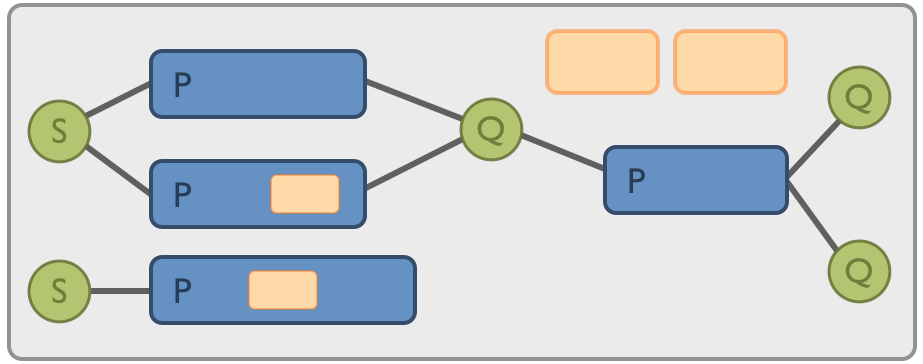
\includegraphics[scale=0.3]{graphics/streams-graph}
  \caption{\label{fig:xmlProcess} The general concept of a data-flow
    graph. The \streams framework provides means for defining streams
    (S), connected processes (P), queues (Q) and adds an abstract
    orthogonal control flow layer (orange elements).}
\end{figure}

In this section we introduce the basic concepts and ideas that we
model within the \streams framework. This mainly comprises the data
flow), the control flow (anytime services) and the basic data
structures and elements used for data processing. The objective of the
abstraction layer is to provide a simple means for rapid prototyping
of data stream processes and a clean and easy-to-use API to implement
against.

The structure of the \streams framework builds upon three aspects:
\begin{enumerate}
\item A {\em data representation} which provides a modeling of the
  data that is to be processed by the designed stream processes
\item Elements to model a {\em data flow}
\item A notion of {\em services} which allow for the implementation
  of {\em anytime service} capabilities.
\end{enumerate}
All of these elements are provided as simple facades (interfaces)
which have default implementations. The abstraction layer provided by
these facades is intended to cover most of the use cases with its
default assumptions, whereas any special use cases can generally be
modeled using a combination of different building blocks of the API
(e.g. queues, services) or custom implementations of the facades.

\subsection*{\label{sec:xmlToRuntime}Executing Data Flow Graphs}
The main objective of the \streams framework is to provide an adequate
abstraction layer, which enables users to design streaming processes
without the need to write any code. A user can prototype {\em
  containers}, which are the top-level elements containing a data flow
graph built from the base elements {\em stream}, {\em process} and
{\em queues}. The {\em process} elements are the executing instances
which need to be enriched with functions ({\em processors}) that do
the actual work. The framework provides a large set of such processors
that can be used to add the required functionality into the data flow
graph. The containers (graphs) are defined in XML.

The XML process definitions are designed to be independent of the
underlying execution platform. The \streams framework provides its own
default runtime implementation, which is able to execute the XML data
flow graphs. This {\em streams} runtime is a Java library with a very
small footprint (less than 200 kilobytes) that can be instantly executed on any
Java VM.

In addition, \streams provides a compiler to map XML process
definitions to {\em Storm} topology, to execute processes on a Storm
cluster. A third execution engine is provided for the Android
platform, which allows for running \streams definitions on mobile
devices that are powered by the Android operating system.\baustelle


\begin{figure}[h!]
  \centering
  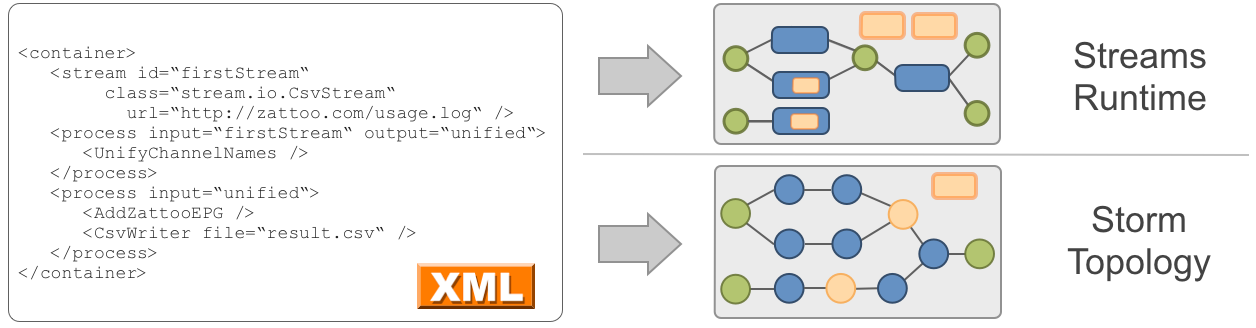
\includegraphics[scale=0.3]{graphics/compile-xml}
  \caption{\label{fig:compileXml}The XML is compiled into a data flow
    graph for different runtime environments. Currently the \streams
    runtime is supported and a prototype for the {\em Storm} compiler
    exists.}
\end{figure}


\subsection{\label{sec:data}Data Representation and Streams}
A central aspect of data stream processing is the representation of
data items that contain the values which are to be processed. From a
message passing system point of view this is the concrete
representation of messages. The abstraction of the \streams framework
considers the case of continuous streaming data being modeled as a
sequence of {\em data items} which traverse the compute graph.

A data item is a set of $(k,v)$ pairs, where each pair reflects
an attribute with a name $k$ and a value $v$. The names are required
to be of type {\ttfamily String} whereas the values can be of any
type that implements Java's {\ttfamily Serializable} interface. The
data item is provided by the {\ttfamily stream.Data} interface.

\begin{table}[h!]
\centering
{
\renewcommand{\arraystretch}{1.25}
\begin{tabular}{c|c}\hline
\textsf{\textbf{Key}} & \textsf{\textbf{Value}} \\ \hline \hline
{\ttfamily x1} & {\ttfamily 1.3} \\ \hline
{\ttfamily x2} & {\ttfamily 8.4} \\ \hline
{\ttfamily source} & {\ttfamily "file:/tmp/test.csv"}  \\ \hline
\end{tabular}
}
\caption{\label{tab:dataitem}A data item example with 3 attributes.} 
\end{table}

Table \ref{tab:dataitem} shows a sample data item as a table of
(key,value) rows. This representation of data items is provided
by hash tables, which are generally provided in almost every modern
programming language.

The use of such hash tables was chosen to provide a flexible data
structure that allows for encoding a wide range of record type as well
as supporting easy interoperation when combining different programming
languages to implement parts of a streaming process. This enables the
use of languages like Python, Ruby or JavaScript to implement custom
process as we will outline in more detail in Section
\ref{sec:scripting}.

\subsection*{Streams of Data}
A {\em data stream} in consequence is an entity that provides access
to a (possibly unbounded) sequence of such data items. Again, the
\streams abstraction layer defines data streams as an interface, which
essentially provides a method to obtain the next item of a stream.

\begin{figure}[h1]
  \begin{center}
    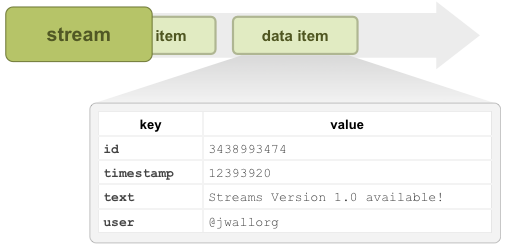
\includegraphics[scale=0.5]{graphics/stream-items.png}
  \end{center}
  \caption{\label{fig:datastream}A {\em data stream} as a sequence of {\em data item} objects.}
\end{figure}

The core \streams library contains several implementations for data
streams that reveal data items from numerous formats such as CSV data,
SQL databases, JSON or XML formatted data. A list of the available
data stream implementations is available in the appendix \ref{app:dataStreams}.

In addition, application specific implementations for data streams can
easily be provided by custom Java classes, as is the case in the FACT
telescope data use-case outlined in section \ref{sec:fact}.

%Throughout this work, we will denote a {\em
%  data stream} by $D$ and a family of such streams as $D_l$. A data
%stream $D$ is a sequence
%\begin{displaymath}
%  D = \langle d_0,d_1,\ldots,d_i,\ldots \rangle
%\end{displaymath}
%of data items $d_i$. Let $A = \{A_1,\ldots,A_p\}$ be a set of
%attributes, then a data item $d_i$ is a function mapping attributes to
%values of a domain associated with each attribute. In database
%notation, each $d_i$ is a tuple of $M^p = M_{A_1} \times\ldots\times
%M_{A_p}$ for sets $M_j$. The $M_j$ can be any discrete sets of a fixed
%domain as well as $M_j \subseteq \mathbb{R}$. The values of each data
%item are further denoted by $d_i(k)$, i.e.
%\begin{displaymath}
%  d_i = ( d_i(A_1),\ldots,d_i(A_p) ).
%\end{displaymath}
%
%The index $i$ may reflect some time unit or a (monotonically
%increasing) time-like dimension, constituting the sequence of
%tuples. For $p=1$ and $M_1 = \mathbb{R}$ this models a single value
%series with index $i$.


%
%. The {\em data items} $s_i$ are tuples of
%$M^p$ with $p \ge 1$ where $M^p = M_1 \times \ldots \times M_p$ for
%any sets $M_j$. 
%

\subsection{\label{sec:basics}Processes and Processors}
The {\em data stream}s defined above encapsulate the format and reading
of data items from some source. The \streams framework defines a
{\em process} as the consumer of such a source of items. A process is
connected to a stream and will apply a series of {\em processors} to
each item that it reads from its attached data stream.

Each {\em processor} is a function that is applied to a data item and
will return a (modified or new) data item as a result. The resulting
data item then serves as input to the next processor of the
process. This reflects the pipes-and-filters concept mentioned in the
beginning of this section.

The {\em processors} are the low-level functional units that actually
do the data processing and transform the data items. There exists a
variety of different processors for manipulating data, extracting or
parsing values or computing new attributes that are added to the data
items.  From the perspective of a process designer, the {\em stream}
and {\em process} elements form the basic data flow elements whereas
the processors are those that do the work.

\begin{figure}[h!]
\centering
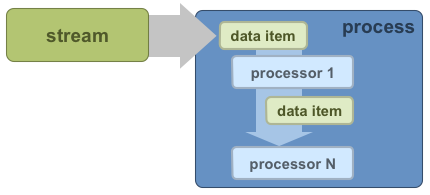
\includegraphics[scale=0.5]{graphics/inside-process.png}
\caption{\label{fig:process}A process reading from a stream and applying processors.}
\end{figure}

The simple setup in Figure \ref{fig:process} shows the general role of
a process and its processors. In the default implementations of the
\streams library, this forms a {\em pull oriented} data flow pattern
as the process reads from the stream one item at a time and will only
read the next item if all the inner processors have completed. 

Where this pull strategy forms a computing strategy of {\em lazy
  evaluation} as the data items are only read as they are processed,
the \streams library is not limited to a {\em pull oriented} data
flow.
% We discuss the implementation of {\em active streams} and the
%resulting {\em push} oriented data flow in Section \ref{sec:push}.


\subsection*{Using multiple Processes}
In the \streams framework, processes are by default the only executing
elements. A process reads from its attached stream and applies all
inner processors to each data item. The process will be running until
no more data items can be read from the stream (i.e. the stream
returns {\ttfamily null}). Multiple streams and processes can be
defined and executing in parallel, making use of multi-core CPUs as
each process is run in a separate thread\footnote{This is the default
  behavior in the reference \streams runtime implementation. If
  \streams processes are executed in other environments, thus behavior
  might be subject to change.}.

For communication between processes, the \streams environment provides
the notion of {\em queues}. Queues can temporarily store a limited
number of data items and can be fed by processors. They do provide
stream functionality as well, which allows queues to be read from by
other processes.

Figure \ref{fig:queues} shows two processes being connected by a
queue. The enlarged processor in the first process is a simple {\em
  Enqueue} processor that pushes a copy of the current data item into
the queue of the second process. The second process constantly reads
from this queue, blocking while the queue is empty.

\begin{figure}[h!]
  \begin{center}
    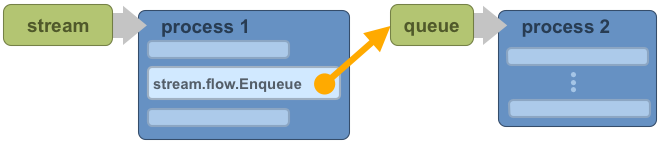
\includegraphics[scale=0.5]{graphics/process-queues.png}
  \end{center}
  \caption{\label{fig:queues}Two Processes $P_1$ and $P_2$ communicating via queues.}
\end{figure}

\bigskip

These five basic elements ({\em stream}, {\em data item}, {\em
  processor}, {\em process} and {\em queue}) already allow for
modeling a wide range of data stream processes with a sequential and
multi-threaded data flow. Apart from the continuous nature of the data stream source, this model
of execution matches the same pipelining idea known from tools like
RapidMiner, where each processor (operator) performs some work on a
complete set of data (example set).
%This contrasts to the current RapidMiner execution model, where each
%operator within a process is executed only once (not counting loops as
%within a cross validation).
%This simple {\em data flow} view serves as the basic data-driven
%exectuion model. 

\subsection{Data Flow and Control Flow}
A fundamental requirement of data stream processing is given by the
{\em anytime paradigm}, which allows for querying processors for their
state, prediction model or aggregated statistics at any time. We will
refer to this anytime access as the {\em control flow}.  Within the
\streams framework, these anytime available functions are modeled as {\em
  services}. A service is a set of functions that is usually provided
by processors and which can be invoked at any time. Other processors
may consume/call services. 

This defines a control flow that is orthogonal to the data flow. Whereas
the flow of data is sequential and determined by the data source, the
control flow represents the anytime property as the functions of services
may be called asynchronous to the data flow.
Figure \ref{fig:control} shows the flow of data and service access.

Examples for services my be classifiers, which provide functions for
predictions based on their current state (model); static lookup
services, which provide additional data to be merged into the stream
or services that can be queried for current statistical information
(mean, average, counts).

\begin{figure}[h!]
  \begin{center}
    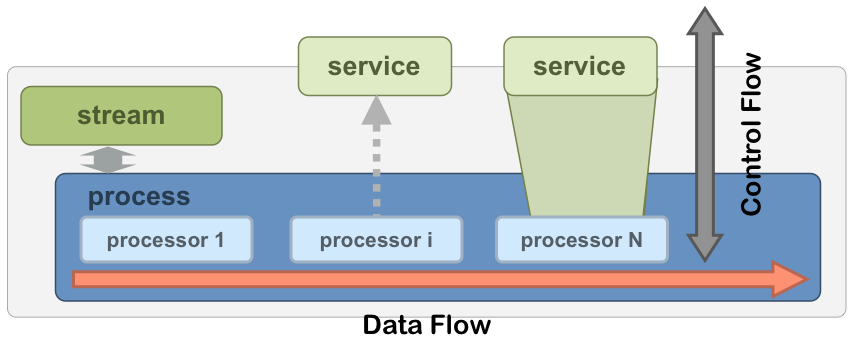
\includegraphics[scale=0.35]{graphics/data-control-flow.png}
  \end{center}
  \caption{\label{fig:control}Orthogonal {\em data} and {\em control
      flow}. Processors may use services as well as export
    functionality by providing services.}
\end{figure}

\subsubsection*{Service References and Naming Scheme}
In order to define the data flow as well as the control flow, a naming
scheme is required. Each service needs to have an unique identifier assigned
to it. This identifier is available within the scope of the experiment and
will be used by service consumers (e.g. other processors) to reference that
service.

At a higher level, when multiple experiments or stream environments are running
in parallel, each experiment is associated with an identifier by itself. This
imposes a hierarchical namespace of experiments and services that are defined
within these experiments. The {\em streams} library constitutes a general
naming scheme to allow for referencing services within a single experiment
as well as referring to services within other (running) experiments.

A simple local reference to a service or other element (e.g. a queue) is 
provided by using the identifier (string) that has been specified along with
the service definition. Following a URL like naming format, services within
other experiments can be referenced by using the experiment identifier and
the service/element identifier that is to be referred to within that experiment,
e.g.
\begin{displaymath}
  \mbox{\ttfamily //experiment-3/classifier-2}.
\end{displaymath}
Such names will be used by the \streams library to automatically resolve references
to services and elements like queues.




%
%
%\subsection{Service Registration and Lookup}
%Each service defined within a process needs to have an unique
%identifier assigned to it. This identifier is used to reference that
%service, e.g. from a processor.

%%It is also possible to define standalone services, e.g. for lookup
%%tables on static data. Processors may also consume services.  
%%\subsubsection*{Using Services for Test-then-Train Evaluation}
%A simple example is given by a learning algorithm (classifier). This
%can process data items as part of its learning process. It provides a
%{\em PredictionService}, which contains as single {\ttfamily predict}
%function. This function uses the current prediction model of the
%learning algorithm to return a prediction for a data item. 

%Figure \ref{fig:control} shows the {\em Naive Bayes Learner} embedded
%into a process. This process implements the {\em test-then-train}
%methods for evaluating stream classifiers on labeled data
%streams. Each item of the stream is first used for testing by making a
%prediction for that item, and then used for updating the prediction
%model.

%The first processor {\em Add Prediction} in this process uses the
%prediction service provided by the {\em Naive Bayes Learner} to make
%a prediction for each data item. After the prediction, the item is
%handed over to the learner, which incorporates it into its model.

%After these two processors, the data item contains the original, true
%label, and the prediction added by the {\em Add Prediction} processor.
%The {\em Prediction Error} processor can now apply any loss function
%to determine the prediction error and aggregate that error over time.

%\subsection{Multiple Processes}
%Often, applications require multiple streams and processes to run
%simultaneously. Following this objective, services of processes can be
%accessed from within other processes whereas queues can serve as
%inter-process communication media and synchronization tool.

